\section{10/8/2019}

\subsection{Resilience Beyond Mean Estimation}

Recall our general framework for robust statistics
(\cref{fig:robust-statistics-framework}, reproduced below):
\begin{figure}[H]
    \centerline{
        \xymatrix{
            \txt{train \\ $\tilde{p}$} \ar[d] \ar@{<->}[r]^-{D(\tilde{p}, p^*) \leq \eps} \ar[dr]
            & \txt{test\\$p^* \in \cG$} \ar[dr] \\
            \txt{$X_1, \ldots, X_n$\\samples} \ar[r] &
            \txt{$\hat\theta(\tilde{p})$\\estimator} \ar[r] &
            \txt{$L(p^*, \hat\theta)$\\loss}
        }
    }
\end{figure}
So far we have only considered mean estimation where
the discrepancy $D = \TV$ and the loss
$L(p, \theta) = \|\theta - \mu(p)\|_2$.
In this section, we will continue to take $D = \TV$ but will
now consider more general losses. Developing this theory will
require suitable generalizations of:
\begin{itemize}
  \item Modulus of continuity
  \item Resilience
  \item Analogue of $\cG_{\Cov}(\sigma)$
    \begin{itemize}
      \item Moment estimation
      \item Linear regression
    \end{itemize}
\end{itemize}


For now, assume $n = \infty$ so we neglect finite sample issues
and our estimator $\hat\theta(\tilde{p})$ directly uses the
corrupted population distribution $\tilde{p}$.

\begin{example}
  $D = \TV$ and $L(p, \theta) = \|\theta - \mu(p)\|_2$
  is the previous mean-estimation framework considered in previous sections.

  For second-moment estimation, we can consider the loss function
  \begin{align}
    L(p, \underbrace{S}_{\in \RR^{d \times d}}) = \|S - \ex_p[X X^\top] \|
  \end{align}
  However, the operator norm is only sensitive to the top eigenspace
  so other times a more natural loss is
  \begin{align}
    \|I - \Sigma^{-1} \Cov_p[X]\|_F
  \end{align}
  Here, the Frobenius norm now weights all eigenvalues equally.

  In linear regression, we will consider the \emph{excess squared loss}
  \begin{align}
    L(p, \theta) = \ex_{(x,y) \sim p}[(y - \braket{\theta, x})^2 - (y - \braket{\theta^*(p), x})^2]
  \end{align}
\end{example}

\subsubsection{Generalizing the modulus of continuity bound}

\myref{prop:mdf-modulus-error-bound}
generalizes naturally: define the modulus of continuity
\begin{align}
  \fm(\cG, 2\eps, L) &= \sup_{\substack{p, q \in \cG \\ \TV(p,q) \leq 2 \eps}}
  L(p, \theta^*(q))
\end{align}
This modulus bounds the minimax loss (i.e.\ worst loss for minimum distance functional),
or more precisely:
\begin{proposition}
  Let the minimum distance functional (MDF) be
  \begin{align}
    \hat\theta(\tilde{p}) = \theta^*(q)~\text{where}~q = \argmin_{q \in \cG} \TV(\tilde{p}, q)
  \end{align}
  Then
  \begin{align}
    \TV(p^*, q) &\leq 2 \eps \\
    L(p^*, \theta^*(q)) &\leq \fm(\cG, 2 \eps)
  \end{align}
\end{proposition}

\begin{proof}
  By assumption, $p^* \in \cG$ and $\TV(\tilde{p}, p^*) \leq \eps$.
  Since $q$ is the minimum-$\TV$-distance projection of $\tilde{p}$
  onto $\cG$, $\TV(q, p^*) \leq \eps$ and by the triangle inequality
  \begin{figure}[H]
    \begin{center}
      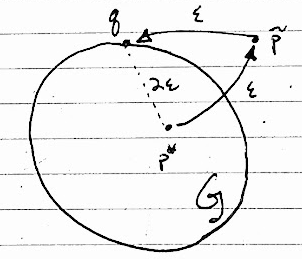
\includegraphics[width=0.4\textwidth]{figures/10-8-1.png}
    \end{center}
  \end{figure}
  We have that $\TV(p^*, q) \leq 2 \eps)$.
\end{proof}

\subsubsection{Resilience}

Resilience is less trivial.  Recall
from \myref{def:resilience} that
$p$ is $(\rho, \eps)$-resilient if
\begin{align}
  \|\mu(p) - \mu(r)\|_2 \leq \rho~\text{whenever}~r \leq \frac{p}{1-\eps}
\end{align}
Our argument for robust mean estimation for $p^* \in \cG_{\TV}$
relied on (1) the existance of a midpoint distribution, and
(2) the triangle inequality. A sketch of the argument is below:
\begin{lemma}
  If $\TV(p, q) \leq \eps$, there is a \emph{midpoint} $r$ such that
  $r \leq \frac{p}{1-\eps}$, $r \leq \frac{q}{1-\eps}$.
\end{lemma}

\begin{figure}[H]
  \begin{center}
    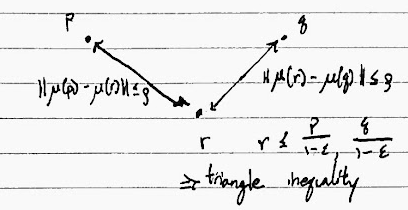
\includegraphics[width=0.4\textwidth]{figures/10-8-2.png}
  \end{center}
  \caption{For resilient distributions, $\fm(\cG_{\TV}, \eps) \leq 2 \rho$.}
  \label{fig:res-dist-mdf-triangle}
\end{figure}

While so long as $D = \TV$ we still have \cref{lem:midpoint},
more general losses $L(p, \theta)$ may not satisfy the triangle inequality.
Handling this requires the following generalized definition for resilience:

\begin{definition}[Resilience for general losses]\label{def:resilience-general}
  $p$ is \emph{$(\rho_1, \rho_2, \eps)$-resilient (for general $L$)} if
  all of the following hold:
  \begin{description}
    \item[Downwards condition $\cG_\downarrow$]
      $L(r, \theta^*(p)) \leq \rho_1$ for all $r \leq \frac{p}{1-\eps}$.
      So the parameter $\theta^*(p)$ should do well for all $\eps$-deletions $r$.
    \item[Upwards condition $\cG_\uparrow$]
      If $L(r, \theta) \leq \rho_1$ for any $r \leq \frac{p}{1-\eps}$
      and $\theta$, then $L(p, \theta) \leq \rho_2$. So any parameter $\theta$
      which does well on some $\eps$-deletion also does well on $p$.
  \end{description}
\end{definition}

\begin{example}[Compatibility of generalized resilience for mean estimation]
  To see what these conditions imply for the familiar setting of mean
  estimation, take $L(p, \theta) = \|\mu(p) - \theta\|_2$ and
  $\theta^*(p) = \mu(p)$.

  The downward condition requires
  \begin{align}
    L(r, \theta^*(p)) &= \|\mu(r) - \mu(p)\|_2 \\
    \|\mu(r) - \mu(p)\|_2 &\leq \rho_1 \qquad \forall r \leq \frac{p}{1-\eps}
  \end{align}
  In other words, the mean of any $\eps$-deletion $r$ is within $\rho_1$
  of the original mean. This is precisely \myref{def:resilience}
  for $\cG_{\TV}$.

  The upward condition says
  \begin{align}
      \|\mu(r) - \theta\|_2 \leq \rho_1 \implies
      \|\mu(p) - \theta\|_2 \leq \rho_2
  \end{align}
  But notice from the downward condition
  \begin{align}
    \|\mu(p) - \theta\|_2
    \leq \|\mu(p) - \mu(r)\| + \|\mu(r) - \theta\|
    \leq \rho_1 + \rho_1
  \end{align}
  So choosing $\rho_2 = 2 \rho_1$, we see that the downwards condition includes
  the upwards condition.
  Together, we see that generalized resilience is compatible with
  our previous definition for $\cG_{\TV}$. In other words
  \begin{center}
    $(\rho,\eps)$-resilience $\iff$ $(\rho, 2\rho, \eps)$-resilience \end{center}
\end{example}

\begin{definition}
  Let $\cG_{\downarrow}(\rho_1, \eps) = \{\text{ all $p$ satisfying $\downarrow$}\}$,
  $\cG_{\uparrow}(\rho_1, \rho_2, \eps) = \{\text{ all $p$ satisfying $\uparrow$}\}$,
  and
  $\cG_{\TV}(\rho_1, \rho_2, \eps) = \cG_{\downarrow}(\rho_1, \eps) \cap \cG_{\uparrow}(\rho_1, \rho_2, \eps)$.
\end{definition}

The key property of generalized resilience is that this family has a nice modulus
bound:
\begin{proposition}
  $\fm(\cG_{\TV}(\rho_1, \rho_2, \eps), \eps) \leq \rho_2$.
\end{proposition}

\begin{proof}
  Need to show for any $p, q \in \cG_{\TV}$ such that $\TV(p, q) \leq \eps$, we have
  $L(p, \theta^*(q)) \leq \rho_2$.
  Since $D = \TV$, \myref{lem:midpoint} is still applicable so there exists
  some midpoint distribution $r$.
  Consider the following figure:
  \begin{figure}[H]
    \begin{center}
      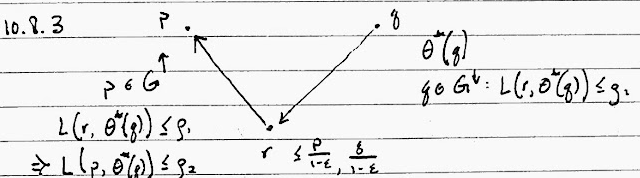
\includegraphics[width=0.7\textwidth]{figures/10-8-3.png}
    \end{center}
    \caption{
      We use $\cG_\downarrow$ to move $q \to r$
      and $\cG_\uparrow$ to move $r \to p$.
      Compare to \cref{fig:res-dist-mdf-triangle},
      where the triangle inequality is used to combine
      resilience bounds between $q \to r$ and $r \to p$
      to control $\|\mu(q) - \mu(p)\|_2$.
  }
  \end{figure}
  Note that $L(r, \theta^*(q)) \leq \rho_1$ since $q \in \cG_\downarrow$,
  and therefore by $\cG_\uparrow$ $L(p, \theta^*(q)) \leq \rho_2$.
\end{proof}

\begin{example}[Second moment estimation]
  Let $L(p, S) = \|S - \ex_p[ X X^\top]\|$.
  The resilience conditions now become:
  \begin{itemize}
    \item
      $\cG_\downarrow(\rho, \eps) \implies \|\ex_r[X X^\top] - \ex_p[X X^\top]\| \leq \rho_1$
      whenever $r \leq \frac{p}{1-\eps}$.
      This is just saying that $X X^\top$ is (old) $(\rho_1, \eps)$-resilient under
      operator norm.

    \item
      $\cG_\uparrow(\rho, \eps) \implies \|\ex_r[X X^\top] - S\| \leq \rho_1$,
      $\rho_2 = 2 \rho_1$, $\implies \|\ex_p[x x^\top] - S\| \leq \rho_2$.
  \end{itemize}
  We will verify these resilience properties when $p$ has bounded moments.

  For $\cG_\downarrow$, $X X^\top$ is $(2 \sigma \sqrt{\eps}, \eps)$-resilient
  in operator norm provided $\Var[\braket{X X^\top, Z}] \leq \sigma^2$ for
  all $\|Z\|_* \leq 1$
  (\cref{eg:bdd-cov-resilient} and \cref{eq:bdd-cov-other-norms}).
  For $\|\cdot\|$ the operator norm, the dual norm is the nuclear norm
  \begin{align}
    \|Z\|_* = \sum_i \sigma_i(Z)
  \end{align}
  where $\sigma_i(Z)$ are the singular values of $Z$.
  For $\|Z\|_* \leq 1$, the extreme points are $\pm v v^\top$
  with $\|v\|_2 = 1$, so we want to show
  \begin{align}
    \Var[\braket{X X^\top, v v^\top}]
    &= \Var[\braket{X, v}^2]
    \leq \ex[\lvert \braket{X, v}^2 \rvert^2]
    = \ex[\braket{x, v}^4]
    \underbrace{\leq}_{\text{WTS}} \sigma^2
  \end{align}
  If we have bounded $4$th moments
  $\ex[\braket{x, v}^4]^{1/4} \leq \tau$,
  then $\sigma = \tau^2$ and we get $(2 \tau^2 \sqrt{\eps}, \eps)$-resilience.

  $\cG_{\uparrow}$ is implied by $\cG_{\downarrow}$ after taking
  $\rho_2 = \rho_1$ and using the same argument as the mean estimation example.

  More generally, for any $k$ and distributional assumptions $\cG_{2k}$ we have
  $(2 \sigma \eps^{1 - 1/k}, \eps)$-resilience for mean estimation
  and $(2 \sigma^2 \eps^{1 - 2/k}, \eps)$-resilience for second moment estimation.
\end{example}

The previous example relied on the symmetry of the loss as well as
triangle inequality of the operator norm, which is not satisfied in the
next setting.

\begin{proposition}[Linear regression]
  Suppose $(X, Y) \sim p$, $L$ is excess squared loss
  \begin{align}
    L(p, \theta) = \ex_{(X,Y) \sim p}[(Y - \braket{\theta, X})^2 - (Y - \braket{\theta^*(p), X})^2]
  \end{align}
  Define the ``noise'' $Z = Y - \braket{\theta^*(p), X}$.
  If
  \begin{description}
    \item[Bounded noise] $\ex[X Z^2 X^\top] \preceq \sigma^2 \ex[X X^\top]$
    \item[Hypercontractivity] $\ex[\braket{X, v}^4] \leq \kappa \ex[\braket{X, v}^2]^2$ for all $v$
  \end{description}
  and $\eps \leq 1/2$, $\eps(\kappa - 1) \leq 1 / 16$, then $p$
  is $(\rho, 8\rho, \eps)$-resilient with $\rho = 3 \sigma \sqrt{\eps}$.
\end{proposition}


\begin{proof}
  Some general observations:
  \begin{itemize}
    \item The loss is a quadratic form in the second moment matrix for $p$, that is:
      \begin{align}
      L(p, \theta)
      &= \ex_p[(y - \braket{\theta, x})^2 - (y - \braket{\theta^*(p), x})^2] \\
      &= (\theta - \theta^*(p))^\top S_p (\theta - \theta^*(p)) \\
      &= \|\theta - \theta^*(p)\|_{S_p}^2
      \end{align}
      where $S_p = \ex_p[X X^\top]$.
    \item An $\eps$-deletion should not change too much in second moment matrix:
      $S_r \approx S_p$
    \item Nor should an $\eps$-deletion change much in mean: $\theta^*(r) \approx \theta^*(p)$
  \end{itemize}

  We first use hypercontractivity to make precise $S_r \approx S_p$:
  \begin{lemma}\label{lem:linreg-second-moment-close}
    If $\eps (\kappa - 1) \leq \frac{1}{16}$, then
    \begin{align}
      \frac{1}{2} S_p \preceq S_r \preceq \frac{3}{2} S_p
    \end{align}
    if $r \leq \frac{p}{1-\eps}$
  \end{lemma}
  \begin{proof}
    As $r$ is an $\eps$-deletion of $p$,
    let $r = p \mid E$ for some event with $p(E) > 1 - \eps$.
    Then by Cauchy-Schwarz and $\eps \leq 1/2$, we have
    (note similarity between this proof and that for \cref{corr:mod-cont-cov})
    \begin{align}
      v^\top S_p v - v^\top S_r v
      &= \lvert \ex_p[\braket{X,v}^2] - \ex_r[\braket{X,v}^2]\rvert \\
      &= \lvert \ex_p[\braket{X,v}^2] - \ex_p[\braket{X,v}^2 \mid E]\rvert \\
      &= \frac{\left\lvert \ex_{X \sim p}\left[
      \ind_E \left(
        \braket{X, v}^2 - \ex_{X \sim p}[\braket{X, v}^2
    \right)\right] \right\rvert}{p(E)} \\
      &\leq \frac{1}{1-\eps} \sqrt{ \ex[\ind_E^2] \Var_p[\braket{x,v}^2]} \\
      &\leq 2 \sqrt{\eps \Var_p[\braket{x,v}^2]}
    \end{align}
    Furthermore, by hyercontractivity
    \begin{align}
      \Var_p[\braket{x,v}^2]
      &= \underbrace{\ex_p[\braket{x,v}^4]}_{\leq \kappa \ex_p[\braket{x,v}^2]^2}
      - \ex_p[\braket{x,v}^2]^2
    \end{align}
    Hence
    \begin{align}
      \lvert \ex_p[\braket{x,v}^2] - \ex_r[\braket{x,v}^2]\rvert
      &\leq 2 \sqrt{\eps (\kappa - 1)} \ex_p[\braket{x,v}^2]
      \leq \frac{1}{2} \ex_p[\braket{x,v}^2]
    \end{align}
    Hence $\ex_r[\braket{x,v}^2] \in (1/2 \ex_p[\braket{x,v}^2], 3/2
    \ex_p[\braket{x,v}^2])$ for any $v$.
  \end{proof}

  Next we analyze the upwards and downwards conditions for resilience.
  First note $\theta^*(p) = S_p^{-1} \ex_p[ X Y]$ by pseudoinverse formula
  for least squares and
  \begin{align}
    \theta^*(r) - \theta^*(p)
    &= S_r^{-1} \ex_r[X Y] - S_p^{-1} \ex_p[ X Y] \\
    &= S_r^{-1} \ex_r[X Y - X X^\top S_p^{-1} \ex_p[X Y]] \\
    &= S_r^{-1} \ex_r[X (Y - \braket{\theta^*(p), X})] \\
    &= S_r^{-1} \ex_r[X Z] \label{eq:linreg-second-moment-diff-theta-star}
  \end{align}
  Take for granted $\| S_r^{-1/2} \ex_r[X Z]\|_2 \leq 2 \sigma \sqrt{\eps}$
  (will prove next time).
  Starting with $\cG_{\downarrow}$
  \begin{align}
    L(r, \theta^*(p))
    &= \|\theta^*(p) - \theta^*(r)\|_{S_r}^2 \\
    &= (S_r^{-1} \ex_r[X Z])^\top S_r (S_r^{-1} \ex[X Z]) \\
    &=  \ex_r[X Z]^\top S_r^{-1} \ex_r[X Z] \\
    &= \|S_r^{-1/2} \ex_r[X Z]\|_2^2 \\
    &\leq 4 \sigma^2 \eps = \rho
  \end{align}
  For $\cG_{\uparrow}$, we want to show
  \begin{align}
    \|\theta - \theta^*(r)\|^2_{S_r}
    \leq \rho
    &\implies \|\theta - \theta^*(p)\|^2_{S_p} \leq 8 \rho
  \end{align}
  Using triangle inequality on matrix norms,
  applying \cref{lem:linreg-second-moment-close} to replace $S_p$ with $S_r$,
  and using our assumption $\|\theta - \theta^*(r)\|_{S_r}^2 \leq \rho$
  as well as $\cG_\downarrow$ we have
  \begin{align}
    \|\theta - \theta^*(p)\|_{S_p}
    &\leq \|\theta - \theta^*(r)\|_{S_p}
    + \|\theta^*(r) - \theta^*(p)\|_{S_p} \\
    &\leq \sqrt{2} \|\theta - \theta^*(r)\|_{S_r}
    + \sqrt{2} \|\theta^*(r) - \theta^*(p)\|_{S_r} \\
    &\leq \sqrt{2 \rho}
    + \sqrt{2 \rho}
    \leq \sqrt{8 \rho}
  \end{align}
\end{proof}
